\documentclass[12pt]{article}
\usepackage[T2A]{fontenc}
\usepackage[utf8]{inputenc}
\usepackage{amssymb,amsmath}
\usepackage{amsthm}
\usepackage{mathrsfs}
\usepackage[english,russian]{babel}
\usepackage{indentfirst}
\usepackage{graphicx}

\renewcommand{\arraystretch}{1.2}

\title{Расчет фазового равновесия}
\author{Шевченко А.В., Цыбулин И.В.}

\newcommand{\pd}[2]{\frac{\partial #1}{\partial #2}}
\let\dividesymbol\div
\renewcommand{\div}{\operatorname{div}}
\newcommand{\grad}{\operatorname{grad}}
\renewcommand{\epsilon}{\varepsilon}
\renewcommand{\geq}{\geqslant}
\renewcommand{\leq}{\leqslant}

\newtheorem{note}{Примечание}[section]

%!!!Внимание!!!
%Будем считать, что "компонент" - слово мужского рода ) (а не компонента - женского). В этом случае, правильное склонение таково:
%Падеж  ед.ч.           мн.ч.
%Им.    компонент       компоненты
%Р.     компонента      компонентов
%Д.     компоненту      компонентам
%В.     компонент       компоненты
%Тв.    компонентом     компонентами
%Пр.    компоненте      компонентах

\begin{document}
\maketitle

\section{Введение}

При численном моделировании течений многокомпонентных смесей во многих случаях необходимо учитывать возможность фазовых превращений \cite{Rozenberg}. При некоторых термобарических условиях смесь может находиться в однофазном состоянии, при других условиях расслаиватья на две и более фаз. Уравнения балансов энергии, импульса и количества компонентов, составляющие математическую модель указанных процессов, в общем случае являются нелинейными \cite{Chen}. Вычислительные алгоритмы для численного интегрирования этих уравнений как правило содержат итерационные процедуры, такие как, метод Ньютона. Так как блок расчета фазового равновесия является частью вычислительного алгоритма для моделирования гидродинамических процессов, к нему предъявляются дополнительные требования. При расчете фазового равновесия кроме молярных долей фаз и их составов необходимо вычислять производные некоторых термодинамических величин (например, молярного объема смеси) по параметрам, которые определяют состояние системы и используются в итерационном процессе. Альтернативой точного вычисления производных является использование их разностных аналогов, однако это существенно увеличивает время расчета.

В общем случае условия фазового равовесия должны быть согласованы с уравнениями состояния фаз многокомпонентной смеси \cite{Batalin, Firoozabadi}. В данной работе рассматривается приближение, когда коэффициенты летучести не зависят от составов фаз (или этой зависимостью можно пренебречь). В этом случае условия фазового равновесие описываются в терминах коэффициентов распределения (констант фазового равновесия), зависящих только от давления и температуры \cite{Orr}. Существует точка зрения что все компоненты в той или иной мере содержаться во всех фазах \cite{Prigozhin}. В данной работе, однако, считается, что часть компонентов не содержится в некоторых фазах. В этом смысле рассматривается ограниченная задача о фазовом равновесии. Компоненты смеси разделяются на два типа: \emph{активные} --- те, которые участвуют в установлении фазового равновесия (для которых определены коэффициенты распределения), и \emph{инертные}, роль которых ограничивается участием в балансе энергии. Принимается что активные компоненты могут образовать три фазы: жидкую (нефтяную), газовую и водную.  Жидкая фаза содержит компоненты, не присутствующие в других фазах (тяжелые нефти) и компоненты, присутствующие в газовой фазе (легкие нефти). Газовая фаза наряду с легкими нефтями сожержит нерастворимые газы (содержащиеся только в газовой фазе) и пары воды $\mathrm{H_2O}$. Водная фаза состоит только из одного компонента $\mathrm{H_2O}$. Количество фаз, на которое расслаивается смесь, заранее неизвестно и определяется термобарическим условиями и составом смеси.

Задача о фазовом равновесии, которая рассматривается в данной работе, состоит в следующем. Заданы молярные концентрации всех компонентов смеси, её молярная энтальпия и давление. Требуется определить на какие фазы расслоится смесь, их молярные доли и составы, а также температуру.

Для расчета фазового равновесия используется тот факт, что при фиксированных давлении, температуре и составе в состоянии равновесия потенциал Гиббса смеси достигает своего минимума. Так как выражение для потенциала Гиббса неизвестно, предлагается использовать потенциал Гиббса модельной смеси, каждая фаза которой является идеальным раствором. Модельный потенциал Гиббса выбирается таким образом, чтобы обеспечить те же константы фазового равновесия, что и в исходной модели, и, как следствие, те же равновесные состояния смеси.

Задача минимизации потенциала Гиббса (при фиксированных температуре, давлении и составе смеси) ставится в пространстве независимых степеней свободы: молярных долей (относительно полного количества молей) $\mathrm{H_2O}$ в водной фазе и легких нефтей в жидкой фазе. Указанные величины  однозначно описывают состояние системы (молярные доли и компонентный состав фаз). Условия минимизации потенциала Гиббса в такой постановке дают критерии фазового равновесия для сосуществующих фаз, а балансы количества молей компонентов (уже учтенные в аналитическом виде потенциала) приводят к уравнениям Речфорда--Райса для молярных долей фаз. Множество, на котором проиходит минимизация ограничено и описывается набором естественных условий неотрицательности молярных долей компонентов.
 
Возможна другая постановка задачи минимизации, в рамках которой в аналитической форме потенциала Гиббса уже учтены условия фазового равновесия. В этом случае условия минимума непосредственно приводят к  уравнениям Речфорда--Райса. В такой постановке задача определения фазового равновесия может быть решена рассмотрением ограниченного числа случаев, выбор одного из которых осуществляется по известным критериям. Однако, если температура сама является неизвестной величиной, алгоритм расчета фазового равновесия существенно усложняется, так как в уравнении теплового баланса участвуют не только активные компоненты, но и инертные. В этом случае отсутствуют простые критерии существования фаз.

При вычислении производных возникает ряд дополнительных проблем. Во-первых, производные перестают существовать на границе области минимизации. Во-вторых, при вариации параметров (температуры, давления, состава) может измениться структура множества ограничений. Эта проблема возникает в случае, когда какие-то компоненты смеси отсутствуют.

Первой проблемы можно избежать, изменив постановку задачи так, чтобы минимум достигался во внутренней точке области. Практически, это реализуется методом внутренних (например, логарифмических) барьеров, которые сводят проблему к задаче безусловной минимизации \cite{Prigozhin}. Более того, для метода внутренней точки наличие логарифмических барьеров является частью алгоритма???. Можно ограничиться некоторым значением амплитуды барьера, при котором его можно считать мало влияющим на решение, и этим самым избежать проблемы достижения границы области. Вторая проблема решается добавлением к смеси малого количества отсутствующих компонентов и их удаления (с коррекцией составов фаз) после расчета фазового равновесия и необходимых производных.

При применении метода внутренних барьеров к задаче минимизации потенциала в первой из описанных выше постановок нарушаются условия фазового равновесия, но сохраняется баланс компонентов смеси. Во второй постановке условия фазового равновесия сохраняют свой вид, но нарушаютя балансы компонентов смеси. Для целей моделирования течений многокомпонентных смесей приоритетным является сохранение балансов компонентов, поэтому рассматривается задача минимизации в первой постановке.

Предлагаемый метод расчета фазового равновесия состоит в следующем:
\begin{enumerate}
    \item Выбор модельного потенциала Гиббса
    \item Модификация потенциала в соответствии с методом логарифмических барьеров
    \item \label{enum:3} Запись условий, необходимых для нахождения стационарной точки модифицированного потенциала при фиксированной температуре
    \item \label{enum:4} Добавление уравнения энтальпии, как неявного уравнения на температуру
    \item \label{enum:5} Совместное решение уравнений пунктов \ref{enum:3} и \ref{enum:4}
    \item Коррекция полученного решения
\end{enumerate}

В результате расчета фазового равновесия в п.\ref{enum:5} предлагаемого алгоритма активные компоненты смеси всегда образуют трехфазную систему. Если система фактически (т.е. с исходным модельным потенциалом Гиббса) находится в одно- или двухфазном состоянии, то молярные доли "паразитных" фаз не должны превышать некоторого порога, регулируемого высотой внутреннего барьера. После коррекции п.6 некоторые фазы могут изчезнуть, но вычисленные в п.5 производные сохраняют смысл.

Предлагаемый метод позволяет единообразно решать все задачи подобного типа, что гарантирует устойчивую работу алгоритма.


%\section{Двухфазное состояние многокомпонентной смеси}
%Рассмотрим смесь из нескольких компонентов при фиксированных давлении $p$ и температуре $T$, находящаяся в жидкой (индекс $L$) и газовой (индекс $G$) фазах. Введем обозначения:
%\begin{itemize}
%	\item $\mu_{i,L}, \mu_{i,G}$ --- химические потенциалы компонента $i$ в фазах $L$ и $G$, соответственно
%	\item $N_{i,L}, N_{i,G}$ --- количество молей компонента $i$, находящихся в фазах $L$ и $G$, соответственно. При этом $N_L = \sum_i N_{i,L}$, $N_G = \sum_i N_{i,G}$ - общее количество молей вещества, находящегося в каждой из фаз.
%	\item $x_i = \dfrac{N_{i, L}}{N_L}$, $y_i = \dfrac{N_{i,G}}{N_G}$ --- мольные доли фаз компонента $i$. При этом $ \displaystyle \sum_i x_i = 1 $, $\displaystyle \sum_i y_i = 1 $.
%\end{itemize}
%
%Будем также считать, что выражение для химических потенциалов в фазах задаются соотношениями, верными для идеальных растворов \cite{Prigozhin}:
%
%\begin{equation}
%\begin{aligned}
%\mu_{i,L} = \mu_{i,L}^0 + RT \ln x_i \\
%\mu_{i,G} = \mu_{i,G}^0 + RT \ln y_i
%\end{aligned},
%\label{eq:hid}
%\end{equation}
%где $\mu_{i,\alpha}^0 = \mu_{i,\alpha}^0(p, T)$ --- химический потенциал чистого вещества $i$, находящегося в фазе $\alpha$ при заданных давлении и температуре.
%
%Потенциал Гиббса для этой системы:
%
%\begin{equation}
%\begin{aligned}
%\Phi = \sum_\alpha \Phi_\alpha = \sum_{i, \alpha}{N_{i,\alpha} \mu_{i,\alpha}} = \sum_i \left(N_{i, L} \mu_{i, L} +
%N_{i, G} \mu_{i, G}\right)
%\end{aligned}
%\label{eq:gibbs}
%\end{equation}
%
%Существует несколько условий фазового равновесия системы, которые являются эквивалентными \textbf{[ссылка]}. Первое --- условие равенства хим. потенциалов во всех фазах (в данном случае $\mu_{i, \alpha} = C_i = const$). Второе --- условие достижения минимума потенциала Гиббса $\Phi$ по мольным долям фаз и фазовым составам, с учетом ограничений $\sum_\alpha N_{i, \alpha} = N_i$. Мы будем пользоваться вторым условием, поскольку оно является более универсальным. При условной минимизации потенциала Гиббса отпадает необходимость рассмотрения случаев, связанных с отсутствием фаз, они соответствуют минимуму на границе области.
%
%Введем функцию Лагранжа:
%\begin{equation}
%\mathscr{L} = \Phi + \sum_i{\xi_i \left[N_i - \sum_\alpha N_{i, \alpha} \right]} \label{eq:lagr}
%\end{equation}
%
%
%Условие экстремума функции Лагранжа \eqref{eq:lagr}, учитывая соотношения \eqref{eq:hid}:
%\[
%\left\{
%\begin{aligned}
%& \pd{\mathscr{L}}{N_{i, \alpha}} = \mu_{i, \alpha} + N_{i, \alpha} \cdot RT \frac{1}{N_{i, \alpha}} - \xi_i = 0, \qquad \alpha=L, G \\
%& \pd{\mathscr{L}}{\xi_i} = N_i - \sum_{\alpha} N_{i,\alpha} = 0
%\end{aligned}
%\right.,\quad\forall i
%\]
%
%Или:
%\begin{equation}
%\left\{
%\begin{aligned}
%& \mu_{i, G}^0 + RT \ln y_i + RT - \xi_i = 0\\
%& \mu_{i, L}^0 + RT \ln x_i + RT - \xi_i = 0\\
%& N_i - \sum_{\alpha} N_{i,\alpha} = 0
%\end{aligned}
%\label{eq:lagr2} \right.,\quad\forall i
%\end{equation}
%
%Вычитая в \eqref{eq:lagr2} первое уравнение из второго, получаем, что в состоянии фазового равновесия выполняется условие:
%
%\begin{equation}
%\frac{y_i}{x_i} = \exp \left(\frac{\mu_{i, L}^0 - \mu_{i, G}^0}{RT}\right) = K_i(p,T), \label{eq:lnK}
%\end{equation}
%где $K_i(p,T) \equiv \dfrac{y_i}{x_i}$ --- константа равновесия для компонента $i$.
%
%
%\begin{note}
%Обратите внимание на то, что выражение \eqref{eq:lnK} можно было получить напрямую из условия $\mu_1 = \mu_2$.
%\end{note}
%

\section{Постановка задачи и допущения}

В этом разделе рассматривается вспомогательная задача о нахождении фазового равновесия при фиксированных давлении и температуре. Цель этого раздела --- переформулировать проблему в форме задачи условной минимизации.

Рассматривается многокомпонентная система, которая может расслаиваться на несколько фаз. Часть из компонентов (инертные) не участвует в фазовых превращениях и формирует инертные фазы. Другие компоненты (активные) могут потенциально образовывать три подвижные фазы: жидкую (нефтяная) фазу ( индекс $L$), газовую фазу (индекс $G$) и водную фазу (индекс $W$).

Предполагается следующее распределение компонентов по фазам:
\begin{itemize}
\item Один компонент $\mathrm{H_2O}$ --- может присутствовать в водной и газовой фазах.
\item Легкие нефти --- могут присутствовать в жидкой и газовых фазах. Всего таких компонентов --- $N_{LO}$ (например, $\mathrm{C_5H_{12}}$ в примере, рассмтренном ниже).
\item Тяжелые нефти --- могут присутствовать только в жидкой фазе. Всего --- $N_{HO}$ компонентов.
\item Нерастворимые газы --- могут присутствовать только в газовой фазе. Всего --- $N_{G}$ компонентов.
%\item $N_{S}$ компонентов --- инертные компоненты-фазы --- существуют каждая в своей фазе.
\end{itemize}

Вводятся обозначения (все молярные доли рассматриваются по отношению к количеству молей $N$ всей смеси активных и инертных компонентов):
\begin{itemize}
\item $\lambda, \omega, \gamma$ --- молярные доли в смеси жидкой, водной и газовой фаз соответственно. При этом $\lambda + \omega + \gamma \ne 1$, т.к. учитываются также инертные фазы.
\item $c_0$ - молярная доля $\mathrm{H_2O}$ в смеси
\item В водной фазе находится только $\mathrm{H_2O}$, а значит $\omega$ является также молярной долей $\mathrm{H_2O}$ в водной фазе
\item $\lambda_i = \lambda x_i, \: i = 1 \dividesymbol N_{LO}$ --- молярные доли (относительно полного состава смеси) легких нефтей в жидкой фазе; $x_i$ --- молярные доли легких нефтей в жидкой фазе
\item $c_i, \: i = 1 \dividesymbol N_{LO}$ --- молярные доли легких нефтей в смеси
\item $c_i, \: i = N_{LO} + 1 \dividesymbol N_{LO} + N_{HO}$ --- молярные доли тяжелых нефтей в смеси
\item $c_i, \: i = N_{LO} + N_{HO} + 1 \dividesymbol N_{LO} + N_{HO} + N_G$ --- молярные доли нерастворимых газов
\item $c_i, \: i = N_{LO} + N_{HO} + N_G + 1 \dividesymbol N_{LO} + N_{HO} + N_G + N_S$ --- молярные доли инертных компонентов, которые также являются молярными долями соответствующих фаз

\end{itemize}

В таблице \ref{t:compphases} приведен пример распределения компонентов по фазам. Компоненты $\mathrm{C_5H_{12}}$ и $\mathrm{C_{10}H_{22}}$ считаются легкими нефтями, компонент $\mathrm{C_{15}H_{32}}$ --- тяжелой нефтью. В смеси присутствуют три нерастворимых газа ($\mathrm{N_2}$, $\mathrm{CO_2}$ и $\mathrm{O_2}$), а также два инертных компонента-фазы ($\mathrm{Sand}$ и $\mathrm{Gran}$)

\begin{table}[ht!]
\centering
\begin{tabular}{c|c|c|c|c|c|c}
\multicolumn{1}{c}{$\diagdown$}& \multicolumn{1}{c}{L (нефть)}& \multicolumn{1}{c}{G (газ)}& \multicolumn{1}{c}{W
(вода)}& \multicolumn{1}{c}{S (песчаник)}& Gr (гранит)&
$\sum$\\
\cline{2-6}
$\mathrm{H_2O}$& & $c_0 - \omega$ & $\omega$ & & & $c_0$\\
\cline{1-6}
$\mathrm{C_5H_{12}}$& $\lambda_1$ & $c_1 - \lambda_1$ & & & & $c_1$\\
\cline{2-6}
$\mathrm{C_{10}H_{22}}$& $\lambda_2$ & $c_2 - \lambda_2$ & & & & $c_2$\\
\cline{1-6}
$\mathrm{C_{15}H_{32}}$& $c_3$ & & & & & $c_3$\\
\cline{1-6}
$\mathrm{N_2}$& & $c_4$ & & & & $c_4$\\
\cline{2-6}
$\mathrm{CO_2}$& & $c_5$ & & & & $c_5$\\
\cline{2-6}
$\mathrm{O_2}$& & $c_6$ & & & & $c_6$\\
\cline{1-6}
$\mathrm{Sand}$& & & & $c_7$ & & $c_7$\\
\cline{2-6}
$\mathrm{Gran}$& & & & & $c_8$ & $c_8$\\
\cline{1-6} \multicolumn{1}{c}{$\sum$}& \multicolumn{1}{c}{$\lambda$}& \multicolumn{1}{c}{$\gamma$}&
\multicolumn{1}{c}{$\omega$}& \multicolumn{1}{c}{$c_7$}& \multicolumn{1}{c}{$c_8$}&
\multicolumn{1}{c}{$1$}\\
\end{tabular}
\caption{Пример распределения компонентов по фазам} \label{t:compphases}
\end{table}

Требуется найти количество фаз, на которое расслоится смесь, молярные доли этих фаз и их состав, при известных молярных долях компонентов $c_i, \; i = 0 \dividesymbol N_{LO} + N_{HO} + N_{G} + N_{S}$ и констант фазового равновесия $K_i (p, T), i = 0 \dividesymbol N_{LO} $. Здесь неизвестными величинами являются молярная доля водной фазы $ \omega $ и молярные доли легких нефтей в жидкой фазе $ \lambda_i $ --- всего $N_{LO} + 1$ неизвестная.

В термодинамическом плане указанную проблему можно сформулировать в виде задачи условной минимизации потенциала Гиббса. Так как потенциал Гиббса указанной системы неизвестен, предлагается рассматривать подвижные фазы как идеальные растворы, с параметрами подобранными таким образом, чтобы получить заданные константы фазового равновесия. В этом случае равновесные состояния исходной и модельной систем совпадают.

После исключения несущественных слагаемых (зависящих только от $p$ и $T$), модельный потенциал Гиббса принимает вид:

\begin{equation}
\begin{aligned}
{\phi} &= \omega \varkappa_0 + \sum_{i=1}^{N_{LO}} \lambda_i \varkappa_i + \sum_{i=1}^{N_{LO}} L(\lambda_i) - L(\lambda) + \\
&+ L(c_0 - \omega) + \sum_{i=1}^{N_{LO}} L(c_i - \lambda_i) - L(s - \lambda - \omega)
\end{aligned}
\label{eq:pproblem}
\end{equation}

Минимум функции $\phi$ ищется при ограничениях:

\begin{equation}
\left\{
\begin{aligned}
0& \leq \omega \leq c_0\\
0& \leq \lambda_i \leq c_i, \qquad i = 1,2,\dots,N_{LO}
\end{aligned}
\right. \label{eq:restr}
\end{equation}

Здесь
\begin{itemize}
\item $\varkappa_i = \ln K_i(p, T)$ --- логарифмы констант равновесия 
\item $L(x) \equiv x \ln x$
\item $\lambda = \sum_{i=1}^{N_{LO}} \lambda_i$ 
\item $s \equiv \gamma + \lambda + \omega = \operatorname{const}$
\end{itemize}

В общем случае $s \ne 1$, так как задача сформулирована для всех компонентов, а не отдельно для подвижных фаз.



\section{Энтальпия}
Фазовые переходы жидкость-газ в чистых веществах при фиксированном давлении происходят при температуре фазового перехода, определяемой этим давлением. Это обстоятельство приводит к двум проблемам:
\begin{itemize}
\item В некоторых случаях недостаточно знания молярных долей компонентов, давления и температуры для того, чтобы однозначно определить фазовый состав.
\item Зависимость фазовых составов от температуры может содержать разрывы первого рода.
\end{itemize}

Таким образом, для однозначного определения фазового состава требуется дополнительный параметр или соотношение. В данной работе в качестве такого параметра используется молярная энтальпия смеси, фигурирующая в уравнении теплового баланса.

В рассматриваемой задаче молярная энтальпия принимается в виде:
\begin{equation}
\eta = \sum_{i=0}^{N_{LO}+N_{HO}+N_{G}+N_{S}} c_i h_i(p,T) -\omega \Delta h_0(p,T) - \sum_{i=1}^{N_{LO}} \lambda_i
\Delta h_i(p,T) , \label{eq:defenth}
\end{equation}
где $\Delta h_i(p,T)$ --- удельная молярная энтальпия парообразования (положительная величина), а $h_i(p,T)$ --- молярные энтальпии компонентов в ``основной'' фазе. Для $\mathrm{H_2O}$ и легких нефтей, которые участвуют в фазовых переходах, ``основной'' фазой является газовая $G$.

С другой стороны, энтальпия может являться не вспомогательным, а определяющим параметром. Условия фазового равновесия системы (минимизация функционала \eqref{eq:pproblem} по неизвестным $\{\omega, \lambda_i\}$) и соотношение \eqref{eq:defenth} совместно рассматривается как система нелинейных уравнений для определения температуры и соответствующего этой температуре фазового равновесия. Эту систему можно трактовать следующим образом: требуется подобрать такую температуру смеси, чтобы после установления фазового равновесия ее молярная энтальпия равнялась заданной величине.

Отметим, что условие \eqref{eq:defenth} \emph{не является} ограничением в задаче \eqref{eq:pproblem}. Соотношение \eqref{eq:defenth} --- это уравнение на $T$, а блок фазового равновесия --- это неявная функция фазовых составов от температуры.


\section{Метод решения}

Как отмечалось во введении, целью настоящей работы являлось построение алгоритма, рассчитывыющего не только фазовое равновесие, но и производные по независимым переменным --- давлению, температуре, молярным концентрациям компонентов смеси. Проблема состоит в том, что на поверхностях, где изменяется количество фаз, производные не определены. Более того, производные неопределены и в случае отсутствия в смеси того или иного компонента. Для преодоления этих трудностей предлагается произвести коррекцию функционала, состоящую во введении барьеров на границе области минимизации. Этот подход является аналогом метода логарифмических барьеров, который используется для решения задач условной оптимизации.

Барьеры невозможно ввести, если ограничение вырождается в равенство. Поэтому предлагается в начале производить коррекцию молярных долей активных компонентов $c_i \rightarrow c_i + \epsilon_i$. Это соответствует тому, что все компоненты всегда присутствуют при расчете фазового равновесия. После расчета фазового равновесия состав смеси корректируется таким образом, чтобы удалить неприсутствующие исходно компоненты и учесть все ограничения. 

В соответствии с этими рассуждениями произведем коррекцию функционала $\phi$ в \eqref{eq:pproblem} следующим образом:

\begin{equation}
\psi = \phi - \varepsilon \left[ \ln \omega + \ln (c_0 - \omega) + \sum_{i=1}^{N_{LO}} \Big( \ln \lambda_i + \ln (c_i - \lambda_i) \Big) \right]
\end{equation}

Задача минимизации функционала $\phi$ заменяется задачей минимизации функционала $\psi$. Локальный минимум функционала $\psi$ находится строго внутри области вблизи (при достаточно малых $\epsilon$ и $\epsilon_i$) искомого минимума функционала $\phi$. Исходную задачу можно переформулировать в виде: найти минимум функции $\psi$ по переменным $\{\omega, \lambda_i\}$, при условии $\eta(\omega, \lambda_i, T) = h$, где $h$ --- заданное значение молярной энтальпии. Отметим, что последнее условие является не ограничением в задаче минимизации функционала $\psi$ (модельный потенциал Гиббса $\psi$ не минимизируется по температуре $T$), а дополнительным уравнением для определения температуры смеси. Таким образом получаем систему нелинейных уравнений:

\begin{equation}
0 = \mathbf{F}(\mathbf{x}) \equiv
\begin{cases}
 \pd{\psi(\mathbf{x})}{\omega}\\
 \pd{\psi(\mathbf{x})}{\lambda_i}\\
 \eta(\mathbf{x}) - h
\end{cases},
\label{eq:system}
\end{equation}
где $\mathbf{x} = (\omega, \lambda_i, T)$.

Система \eqref{eq:system} далее решается модифицированным методом Ньютона:

\begin{equation}
\left\{
\begin{aligned}
\Delta \mathbf{x}_k &= -\left(\pd{\mathbf{F(\mathbf{x}_k)}}{\mathbf{x}}\right)^{-1}
\mathbf{F}(\mathbf{x}_k)\\
\mathbf{x}_{k+1} &= \mathbf{x}_k + \alpha_k \Delta \mathbf{x}_k\\
\alpha_k &= \min(1, \beta \alpha_{k, \max})
\end{aligned}
\right. \label{eq:newton}
\end{equation}

В методе \eqref{eq:newton} используется ограничитель шага $\alpha_k \leq 1$ для того, чтобы не выйти за границу области определения функции. Когда $\alpha_k = 1$ шаг происходит согласно обычному методу Ньютона. $\alpha_{k, \max} > 0$ --- это максимальное число, такое что $\mathbf{x}_k + \alpha_{k,\max} \Delta \mathbf{x}_{k}$ еще принадлежит области $\omega \in [0,c_0], \lambda_i \in [0, c_i]$, а также выполняется условие $T \in [T_{\min}, T_{\max}]$. Множитель $\beta < 1$ (типично $\beta = 0.9 \dividesymbol 0.99$) используется, чтобы новое приближение было строго внутри области.

Решение задачи можно аналитически продифференцировать по параметрам:

\begin{equation}
\begin{aligned}
&\mathbf{F}(\mathbf{x}(\boldsymbol \alpha), \boldsymbol \alpha) = 0\\
&\pd{\mathbf{F}(\mathbf{x}, \boldsymbol \alpha)}{\mathbf{x}} \pd{\mathbf{x}}{\boldsymbol \alpha} + \pd{\mathbf{F}(\mathbf{x}, \boldsymbol \alpha)}{\boldsymbol \alpha} = 0\\
&\pd{\mathbf{x}}{\boldsymbol \alpha} = -\left(\pd{\mathbf{F}(\mathbf{x}, \boldsymbol \alpha)}{\mathbf{x}}\right)^{-1} \pd{\mathbf{F}(\mathbf{x}, \boldsymbol \alpha)}{\boldsymbol \alpha} \\
\end{aligned}
\end{equation}

\section{Результаты}
Для верификации предложенного алгоритма рассматривалась задача о нахождении фазового равновесия смеси, включающей $\mathrm{H_2O}$ (молярная доля $0.5$) и две легкие нефти: $\mathrm{C_5H_{12}}$ и $\mathrm{C_{10}H_{22}}$ (молярные доли $0.25$). При этом задача решалась в диапазоне температур 530---660~K при давлении $10^7$ Па. На рисунке \ref{fig:1} показаны результаты расчета. 

\begin{figure}
	\centering
	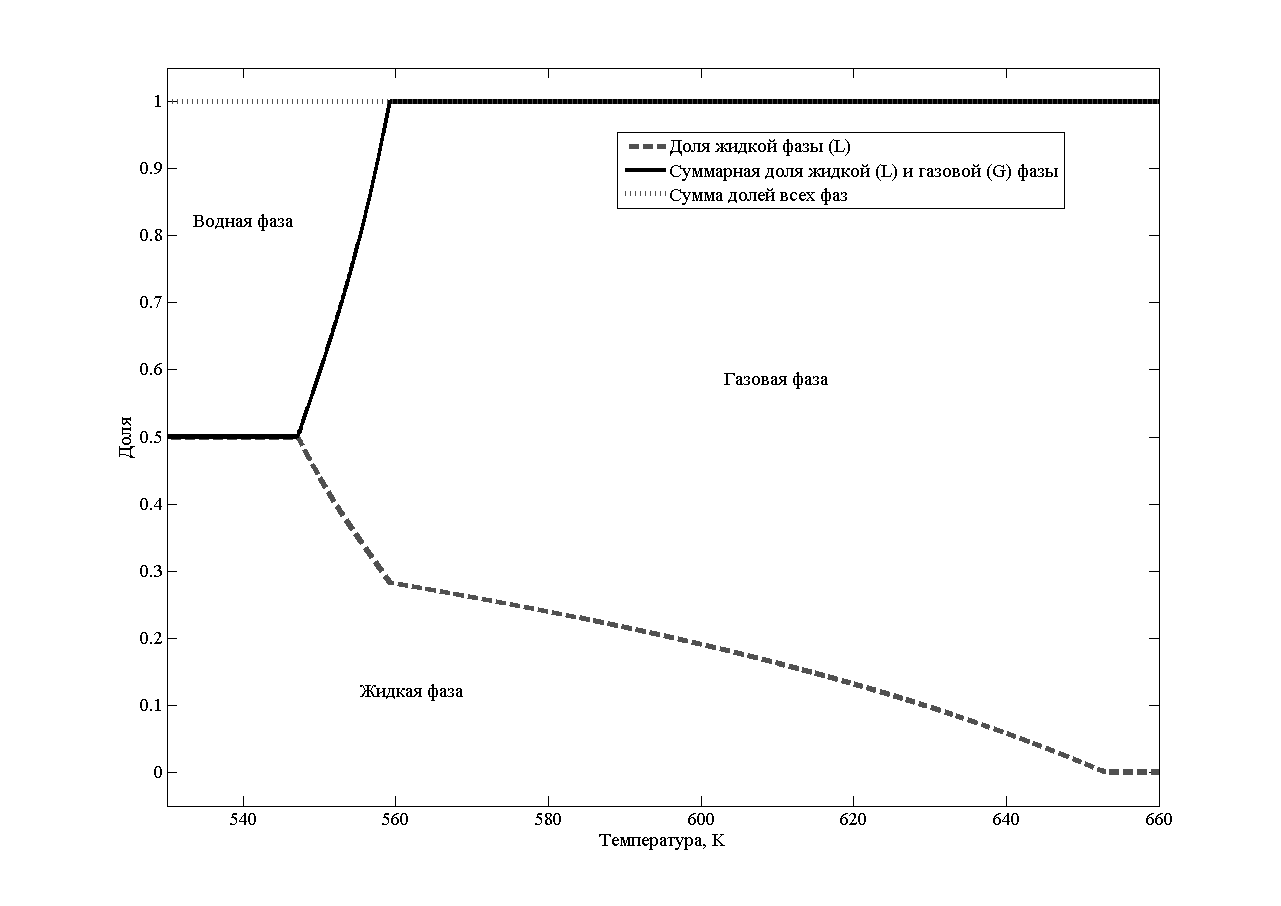
\includegraphics[width=\textwidth]{Figure1.png}
	\caption{График зависимости долей фаз от температуры.}
	\label{fig:1}
\end{figure}

Как видно из графика, большую часть диапазона температур занимают двухфазные состояния (при $T<550$ --- водная и жидкая фазы, а при $T>560$ --- газовая и жидкая). Такие двухфазные состояния равновесия, как отмечалось выше, соответствуют граничным точкам области минимизации потенциала Гиббса и недостижимы в предложенном алгоритме. Однако, визуально построенный график идентичен такому же графику, полученному из ``стандартного алгоритма''. Здесь под ``стандартным'' понимается рассмотрение случаев  фазового состава смеси в состоянии равновесия с точным выполнением соотношений $K_i(p,T) \equiv \dfrac{y_i}{x_i}$ для компонент, которые находятся в нескольких сосуществующих фазах.

Наибольшее отличие результата, полученного предложенным методом, от ``стандартного'' наблюдается в окрестности перехода от двухфазного к трехфазному состоянию (рисунок \ref{fig:2}). Однако, и в этом случае разница невелика~---~она составляет не более~0.5\%.

\begin{figure}
	\centering
	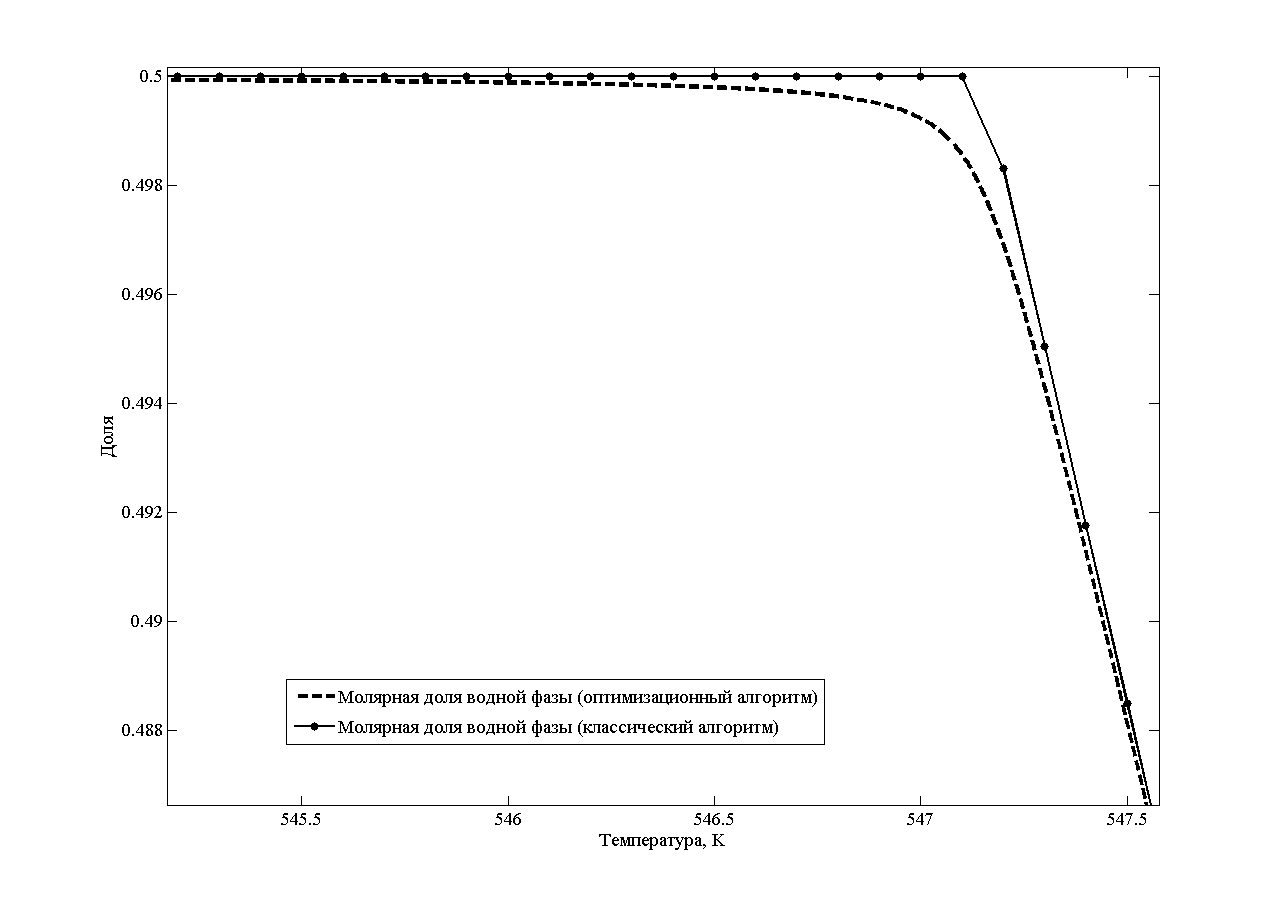
\includegraphics[width=\textwidth]{Figure2.png}
	\caption{Область перехода от двухфазного к трехфазному состоянию.}
	\label{fig:2}
\end{figure}

\section{Выводы}
В данной работе представлен алгоритм расчета задачи о нахождении фазового равновесия смеси нескольких компонент. Алгоритм основывается на методе внутренних логарифмических барьеров и единообразно работает для случаев с разным составом фаз. Проведено сравнение со стандартным алгоритмом нахождения фазового равновесия.


\begin{thebibliography}{9}
    \addcontentsline{toc}{section}{\refname}
    \bibitem{Chen} {\em Chen~Z., Huan~G.,~Ma Y.} Computational Methods for Multiphase Flows in Porous Media //Philadelphia: SIAM --- 2006.
    \bibitem{Prigozhin} {\em Пригожин~И., Дефей~Р.} Химическая термодинамика //Новосибирск: СО изд."Наука. --- 1966.
    \bibitem{Batalin} {\em  Баталин О.Ю., Брусиловский А.И., Захаров М.Ю.} Фазовые равновесия в системах природных углеводородов. --- М.: Недра, 1992.
    \bibitem{Rozenberg} {\em Розенберг~М.~Д., Кундин~С.~А.} Многофазная многокомпонентная фильтрация при добыче нефти и газа //Недра. --– 1976. --– Т. 1. --– С. 320.
    \bibitem{Orr} {\em Orr~F.~M.} Theory of gas injection processes. --– Copenhagen: Tie-Line Publications, 2007.
    \bibitem{Firoozabadi} {\em Firoozabadi~A.} Thermodynamics of hydrocarbon reservoirs. --– New York: McGraw-Hill, 1999.
\end{thebibliography}

\end{document}